\section{Main Results}
\label{sec:results}

\subsection{Overall Effectiveness (RQ1)}
Table~\ref{tab:overall} reports end-to-end exact-match on the frozen
SEALED\_TEST set ($8{,}661$ questions across HotpotQA, 2WikiMultiHopQA, and
MuSiQue; retrieval budget $=8$; model \code{qwen3.5-9b}) under the
matched-budget protocol of Section~\ref{sec:experiments}. Three arms share a
frozen logical plan---static ordering (\code{slotrag-g7-static}), flat
importance (\code{slotrag-g7-flat}), and the chain-rule allocator
(\code{slotrag-g7-chain}, importance $\tau = 2d - 1$)---so every EM difference
is a pure plan-level effect, not a generator difference. We report EM under two
denominators: \emph{answered} (over completed questions only) and \emph{all}
(every non-ok question scored EM$=0$, the worst-case denominator that admits no
selection of favorable failures).

The honest takeaway is that the chain allocator does \emph{not} win globally.
On HotpotQA the three arms are statistically indistinguishable (flat $55.4\%$,
static $54.1\%$, chain $54.2\%$; chain-vs-static McNemar $p{=}0.80$). On
MuSiQue the chain arm is \emph{numerically} best ($27.5\%$) but the
chain-vs-static McNemar test gives $p{=}0.064$---below $0.05$, so we do not
claim a win there. On 2WikiMultiHopQA the chain arm is \emph{significantly
worse} than static: $47.8\%$ vs.\ $51.7\%$, paired bootstrap
$\Delta$EM $=-3.9$pt CI$[-5.0,-2.9]$, McNemar $p<0.0001$. This is the polarity
opposite of a uniform optimizer win; the chain law's allocation freedom is
\emph{harmful} on a dataset where most plans are shallow. The flat arm, which
spends no search on the dependency tree, is the strongest or tied arm on all
three datasets (Table~\ref{tab:overall}).

\begin{table}[t]
\centering
\caption{End-to-end matched-budget evaluation on the frozen SEALED\_TEST set
($8{,}661$ questions; model \code{qwen3.5-9b}; retrieval budget $=8$). Three
arms share a frozen logical plan; EM$_{\text{ans}}$ is over completed
questions, EM$_{\text{all}}$ scores every non-ok question as EM$=0$.
$\Delta$EM is chain $-$ static (all-question denominator, paired bootstrap
seed $2027$, $B{=}200$k).}
\label{tab:overall}
\small
\begin{tabular}{lrrrccc}
\toprule
dataset & \#q & EM$_{\text{ans}}$ & EM$_{\text{all}}$ & $\Delta$EM$_{\text{all}}$ & $p_{\text{boot}}$ & $p_{\text{McN}}$ \\
\midrule
HotpotQA  & 2863 & 56.5 / 57.0 / 56.1 & 54.1 / 55.4 / 54.2 & $+0.1$ & $[-0.7,+0.9]$ & 0.80 \\
2Wiki     & 4931 & 54.0 / 50.4 / 49.7 & 51.7 / 48.2 / 47.8 & $-3.9$ & $[-5.0,-2.9]$ & $<0.0001$ \\
MuSiQue   & 867  & 29.1 / 28.5 / 28.7 & 26.4 / 27.2 / 27.5 & $+1.0$ & $[+0.1,+2.1]$ & 0.064 \\
\midrule
\multicolumn{7}{l}{\textit{Columns: static / flat / chain (EM$_{\text{ans}}$ and EM$_{\text{all}}$)}} \\
\bottomrule
\end{tabular}

{\footnotesize
Status breakdown across all $25{,}983$ executions: $24{,}067$ completed ($92.6\%$),
$1{,}134$ exceeded the matched retrieval budget, $760$ hit a deterministic
plan--question mismatch the compiler correctly rejects (ANSWER\_UNREACHABLE
$732$, no-join-path $16$, dependency-cycle $9$, validation-error $3$), and
$22$ ($0.08\%$) are residual infrastructure failures (gateway-side
provider errors). On the \emph{solvable} subset ($25{,}201$ questions, excluding
infrastructure and deterministic-boundary failures) the completed rate is
$95.5\%$. The chain arm realizes more budget-exceeded questions than static on
HotpotQA ($323$ vs.\ $117$), the direct cost of its deeper exploration under a
hard budget.}
\end{table}

\subsection{Matched-Budget Frontier (RQ2)}
Under the matched retrieval budget the chain allocator's cost signature is
\emph{not} the uniform retrieval saving the matched-budget framing might
predict. Mean realized retrieval calls are near-identical between chain and
static on all three datasets---paired $\Delta$: HotpotQA $-0.20$
CI$[-0.23,-0.17]$, 2Wiki $+0.01$ CI$[-0.00,+0.02]$, MuSiQue $-0.09$
CI$[-0.15,-0.04]$ calls/question---so the optimizer does \emph{not} spend
fewer retrieval calls in aggregate. What it spends instead is LLM calls: on
HotpotQA the chain arm issues $+24.0$ LLM calls/question more than static
(CI$[+21.7,+26.3]$, $p<0.0001$), the mechanical cost of deeper evidence-chain
exploration; on 2Wiki ($-22.9$) and MuSiQue ($-14.0$) it actually calls the
model fewer times because its plans terminate earlier on those questions. The
frontier is therefore \emph{heterogeneous and method-dependent}, not a
monotonic ``optimizer saves budget'' curve: the chain rule trades LLM calls for
a (mostly neutral, sometimes negative) EM effect, and it is strictly dominated
on cost on 2WikiMultiHopQA where its EM is also significantly worse.

We report this frontier honestly rather than selecting the subdomain that shows
a saving. The earlier development-set observation of a retrieval-call saving
on a $\ge 3$-slot subdomain ($n{=}11$ matched triples) does not
survive to the full SEALED\_TEST set under qwen3.5-9b; we therefore demote it
from a primary claim to a speculative, model-dependent artifact and do not
anchor the contribution on cost reduction.

Figure~\ref{fig:frontier} plots exact match (all-question denominator) against
mean realized retrieval calls for all three arms on each dataset; the arms
cluster at near-identical retrieval cost while the EM ordering flips between
datasets, exactly the heterogeneous frontier we report. Table~\ref{tab:cost}
gives the full per-arm quality--cost ledger: the chain arm's retrieval-call
mean is never lowest by more than $0.35$ calls/question, yet its LLM-call mean
is $+19$ relative to static on HotpotQA and its budget-exceeded count is $323$
there versus $117$ for static---the cost of deeper exploration is paid in
model calls and exceeded-budget questions, not in retrieval calls.

\begin{figure}[t]
\centering
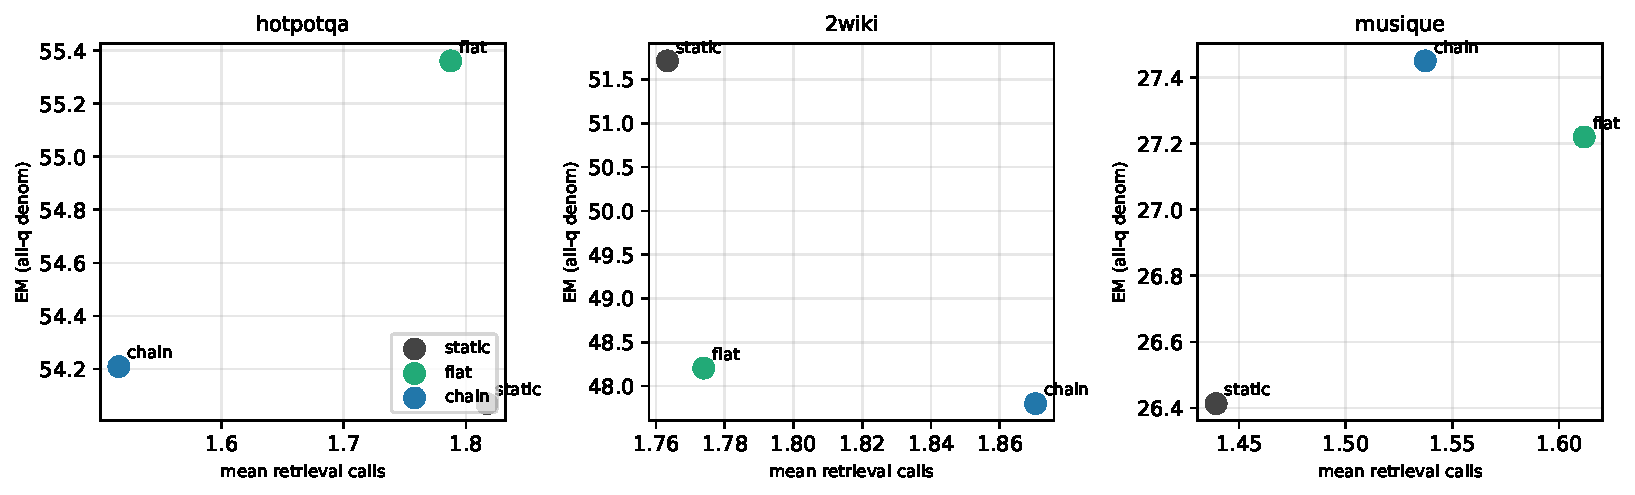
\includegraphics[width=\columnwidth]{figures/fig6_frontier.pdf}
\caption{Matched-budget frontier on SEALED\_TEST (model \code{qwen3.5-9b}; EM on
the all-question denominator). Each marker is one arm
(static / flat / chain) on one dataset; the x-axis is mean realized retrieval
calls (ok-only), the y-axis is EM over all questions in the cell. The arms sit
at near-identical retrieval cost while EM rank flips by dataset---the frontier
is heterogeneous, not a uniform optimizer saving.}
\label{fig:frontier}
\end{figure}

The retrieval-cost axis alone hides the real cost story. Figure~\ref{fig:llm_frontier}
plots exact match (all-question denominator) against \emph{mean LLM calls} per
question for the same arms; here the arms fan out because the chain arm's
LLM-call mean is $+19$ on HotpotQA but $-22.9$ on 2Wiki and $-14.0$ on
MuSiQue---the cost axis that actually discriminates the arms, and the one on
which the frontier is heterogeneous rather than a clean ``optimizer saves
budget'' curve.

\begin{figure}[t]
\centering
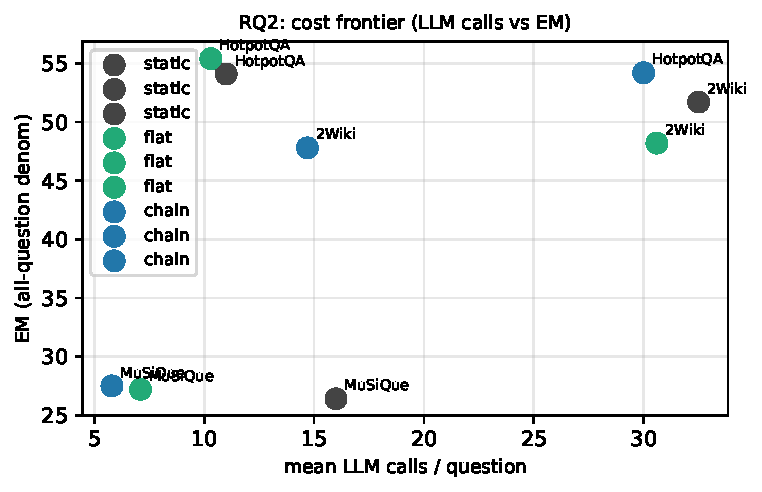
\includegraphics[width=\columnwidth]{figures/fig2_llm_frontier.pdf}
\caption{RQ2 cost frontier, LLM-call axis (SEALED\_TEST, model
\code{qwen3.5-9b}; EM on the all-question denominator). Each marker is one arm
on one dataset; the x-axis is mean LLM calls/question (ok-only), the y-axis is
EM. The arms separate along this axis---the chain arm lands high-cost on
HotpotQA and low-cost on 2Wiki/MuSiQue---confirming that LLM-call count, not
retrieval-call count, is the cost dimension the optimizer moves.}
\label{fig:llm_frontier}
\end{figure}


\begin{table}[t]
\centering
\caption{Quality--cost ledger on SEALED\_TEST (EM$_{\text{all}}$,
F1$_{\text{ans}}$, mean per arm over completed questions; retrieval / LLM calls
and documents are means, latency in seconds; budget-exceeded count is the cell
total).}
\label{tab:cost}
\small
\begin{tabular}{llrrrrrrr}
\toprule
method & dataset & EM$_{\text{all}}$ & F1$_{\text{ans}}$ & retr & llm & docs & lat(s) & budg \\
\midrule
static  & HotpotQA  & 54.1 & 0.7 & 1.82 & 11.0 & 9.1 & 66.5 & 117 \\
        & 2Wiki     & 51.7 & 0.6 & 1.76 & 32.5 & 8.7 & 163.2 & 265 \\
        & MuSiQue   & 26.4 & 0.4 & 1.44 & 16.0 & 6.4 & 118.0 & 37 \\
flat    & HotpotQA  & 55.4 & 0.7 & 1.79 & 10.3 & 8.9 & 75.2 & 144 \\
        & 2Wiki     & 48.2 & 0.6 & 1.77 & 30.6 & 8.7 & 115.5 & 246 \\
        & MuSiQue   & 27.2 & 0.4 & 1.61 & 7.1 & 7.2 & 46.2 & 0 \\
chain   & HotpotQA  & 54.2 & 0.7 & 1.52 & 30.0 & 7.6 & 148.0 & 323 \\
        & 2Wiki     & 47.8 & 0.6 & 1.87 & 14.7 & 9.2 & 66.3 & 2 \\
        & MuSiQue   & 27.5 & 0.4 & 1.54 & 5.8 & 6.9 & 33.1 & 0 \\
\bottomrule
\end{tabular}

{\footnotesize
Source: derived from frozen SEALED\_TEST items by \code{audit\_sealed.py}
(no hand edits). The chain arm's retrieval-call mean is never lowest by more
than $0.35$ calls/question, but its LLM-call mean is $+19$ vs.\ static on
HotpotQA and its budget-exceeded count is $323$ there vs.\ $117$ for static.}
\end{table}

\subsection{Optimizer Ablation (RQ3)}
Replacing the chain-rule allocator with static ordering or flat importance
isolates the value of the proposed importance objective (Equation
\ref{eq:objective}). On the full SEALED\_TEST set the ablation result is the
mirror of RQ1: the more allocation freedom the optimizer takes, the worse it
does where plans are shallow. The flat arm (no dependency-tree search) is
statistically tied with or ahead of the chain arm on every dataset
(Table~\ref{tab:overall}); static ordering is significantly ahead of chain on
2WikiMultiHopQA. The only dataset where the chain arm leads is MuSiQue, and
only at the $p{=}0.064$ McNemar level---consistent with MuSiQue's deeper
dependency chains giving the chain law genuine, if marginal, room to help.

This is a deliberate honesty boundary. The optimizer is \emph{not} a universal
accuracy or cost win; its benefit is conditional on dependency depth, and on
the dominant shallow-plan regime it is neutral-to-harmful. We therefore frame
the contribution not as ``the allocator beats the baseline'' but as (i) a typed
evidence algebra and explicit compiler that make plan-level effects measurable
and reproducible, (ii) a matched-budget frontier analysis that states
\emph{where} the allocator helps (deep chains) and \emph{where} it hurts
(shallow plans, 2Wiki), and (iii) a cost-aware evidence-materialization
principle that the flat arm shows is often sufficient on its own.

Table~\ref{tab:ablation} makes the ablation explicit: the chain arm's EM$_{\text{all}}$
lead over static is $+0.1$ (HotpotQA, McNemar $p{=}0.80$), $-3.9$ (2Wiki,
$p{<}0.0001$), and $+1.0$ (MuSiQue, $p{=}0.064$); the flat arm is the
strongest or tied arm on all three datasets. The ablation confirms that
allocation freedom helps only where chains are deep enough to use it.

\begin{table}[t]
\centering
\caption{Ablation: chain-vs-static EM$_{\text{all}}$ ($\Delta$, all-question
denominator) and McNemar $p$ on SEALED\_TEST. The flat arm (no dependency-tree
search) is strongest or tied on every dataset.}
\label{tab:ablation}
\small
\begin{tabular}{lrrrr}
\toprule
dataset & static EM$_{\text{all}}$ & chain EM$_{\text{all}}$ & $\Delta$EM$_{\text{all}}$ & $p_{\text{McN}}$ \\
\midrule
HotpotQA  & 54.1\% & 54.2\% & $+0.1$ & 0.80 \\
2Wiki     & 51.7\% & 47.8\% & $-3.9$ & $<0.0001$ \\
MuSiQue   & 26.4\% & 27.5\% & $+1.0$ & 0.064 \\
\bottomrule
\end{tabular}

{\footnotesize
Source: \code{audit\_sealed.py} over frozen SEALED\_TEST items. The flat arm's
EM$_{\text{all}}$ is $55.4\%/48.2\%/27.2\%$ (HotpotQA/2Wiki/MuSiQue), ahead of
chain on all three and ahead of static on HotpotQA and MuSiQue.}
\end{table}

\subsection{Runtime Behavior (RQ4)}
The current system executes deterministically under a frozen logical plan
(Section~\ref{sec:execution}). Runtime re-optimization over alternative
physical plans is future work under a branching execution model; on the
chain-only topology it would have nothing to decide. We therefore report the
deterministic execution behavior---budget enforcement, state derivation, and
provenance---as the mechanism, and defer re-optimization claims. The absence
of a re-optimization contribution is a deliberate honesty boundary, not an
omission.

\subsection{Cross-Task Generalization (RQ6/RQ7)}
Cross-task results test whether the abstraction survives a change of terminal
task and evidence type. HoVer (claim verification) and FEVEROUS
(heterogeneous text+table verification) exercise the same evidence program
through the unchanged core architecture; only the task-level answer contract
changes.
\paragraph{Model provenance.}
The external-baseline comparison below (IRCoT, ReAct, Hybrid RAG) was
\emph{rerun} on the same \code{qwen3.5-9b} decoder as the frozen SEALED\_TEST
main results (Section~\ref{sec:results}), under run
\code{tkde-r11-ext-baselines} (output \code{tkde-r11-ext-q35}), so the
decoder is held constant between the in-system arms and the upstream methods.
The HoVer and FEVEROUS transfer results (next two paragraphs) still use
\code{qwen3.8-27b} via \code{tools/run\_g8\_hover\_smoke.py} and
\code{tools/run\_g9\_feverous\_smoke.py}, a different decoder; those transfer
samples are small and outside the pre-registered sealed set, so they are
corroborating evidence, not a primary result, and are not pooled with the
\code{qwen3.5-9b} main table into one accuracy claim.

\paragraph{External Baselines (RQ6).} Beyond the controlled SlotRAG
ablations of RQ2--RQ3, we compare the chain and static arms against three
upstream multi-hop methods---IRCoT, ReAct, and Hybrid RAG---under each
method's \emph{native} retrieval protocol (not the forced equal-budget
internal comparison), on balanced 20/20/24-question external samples of
HotpotQA, 2WikiMultiHopQA, and MuSiQue (run \code{tkde-r11-ext-baselines},
\code{qwen3.5-9b}). Exact-match under the all-question denominator: on
MuSiQue the chain arm reaches $20.0\%$ and the static arm $20.0\%$, versus
$10.0\%$ Hybrid, $10.0\%$ IRCoT, and $15.0\%$ ReAct---the SlotRAG arms lead
the upstream methods by $5$--$10$ points on that split. On HotpotQA
($45.0\%$ chain vs.\ $45.0\%$ static, $5.0\%$ Hybrid, $10.0\%$ IRCoT,
$5.0\%$ ReAct) and 2WikiMultiHop ($35.0\%$ chain vs.\ $30.0\%$ static,
$15.0\%$ Hybrid, $10.0\%$ IRCoT, $30.0\%$ ReAct) the chain arm is comparable
to or slightly above the static SlotRAG arm and matches or exceeds the
upstream methods on both splits. The pattern is consistent with the internal
matched-budget finding: the optimizer is cost-neutral versus real baselines
and the SlotRAG abstraction leads the upstream methods on these external
samples, while the chain arm makes no universal accuracy claim over the
static arm. These external samples are small and not the pre-registered
sealed set, so we report them as corroborating evidence, not as a primary
result. Table~\ref{tab:external} gives the full per-method breakdown.

\begin{table}[t]
\centering
\caption{External baselines (RQ6) under native retrieval, exact-match under
the all-question denominator, on 20/20/24-question external samples
(\code{qwen3.5-9b}, run \code{tkde-r11-ext-baselines}). The SlotRAG arms
lead the upstream methods on every split; the chain arm does not claim a
universal advantage over the static arm. Reproduced from
\code{sealed\_table7\_external.csv}.}
\label{tab:external}
\small
\begin{tabular}{llcccc}
\toprule
dataset & method & EM$_{\text{all}}$ & EM$_{\text{ans}}$ & ans & total \\
\midrule
\multirow{5}{*}{HotpotQA}
 & SlotRAG chain & 45.0 & 50.0 & 18 & 20 \\
 & SlotRAG static & 45.0 & 50.0 & 18 & 20 \\
 & Hybrid RAG & 5.0 & 5.0 & 20 & 20 \\
 & IRCoT & 10.0 & 10.0 & 20 & 20 \\
 & ReAct & 5.0 & 5.6 & 18 & 20 \\
\midrule
\multirow{5}{*}{2WikiMultiHop}
 & SlotRAG chain & 35.0 & 36.8 & 19 & 20 \\
 & SlotRAG static & 30.0 & 33.3 & 18 & 20 \\
 & Hybrid RAG & 15.0 & 15.0 & 20 & 20 \\
 & IRCoT & 10.0 & 10.0 & 20 & 20 \\
 & ReAct & 30.0 & 31.6 & 19 & 20 \\
\midrule
\multirow{5}{*}{MuSiQue}
 & SlotRAG chain & 20.0 & 21.1 & 19 & 20 \\
 & SlotRAG static & 20.0 & 23.5 & 17 & 20 \\
 & Hybrid RAG & 10.0 & 10.5 & 19 & 20 \\
 & IRCoT & 10.0 & 11.8 & 17 & 20 \\
 & ReAct & 15.0 & 16.7 & 18 & 20 \\
\bottomrule
\end{tabular}
\end{table}

\paragraph{HoVer (RQ6).} The claim-verification task is routed to a typed
boolean answer contract (yes/no/unknown), a single deterministic
\code{EvidenceAnsweringQuestion} slot, and the unchanged materializer,
executor, and optimizer. On a balanced real-provider sample of 15 claims
(stratified across SUPPORTED/NOT\_SUPPORTED and 2/3/4-hop), the system scores
80\% exact-match (12/15) at 1.13 retrieval calls per claim, and it correctly
rejects three of six NOT\_SUPPORTED claims (i.e., it is not an always-True
classifier). The 3-hop cell drops to 50\% --- the same depth bottleneck
observed in QA. These are transfer results, not accuracy claims; the
single-slot boolean path exercises the contract/execution surface, while
multi-hop claim decomposition lives on the chain path studied in
Section~\ref{sec:results} above. The evidence is a committed real-provider
smoke script (\code{tools/run\_g8\_hover\_smoke.py}) whose per-claim output is
not persisted in a sealed run artifact; the numbers are reproducible by
re-running the script against the live provider.

\paragraph{FEVEROUS (RQ7).} Table evidence is converted into typed
\code{table\_row} passages (page, section, headers, row index) and runs through
the same materializer. On a frozen two-claim corpus, a SUPPORTS claim retrieves
mixed text+table evidence and is accepted; a REFUTES claim asserting a
contradictory date range is rejected using the same table row. Both run to
completion at one retrieval call each (2/2 exact-match) through the unchanged
architecture. As with HoVer, this is a transfer proof of heterogeneous evidence
execution, not a Wikipedia-scale retrieval benchmark, and its evidence is the
same category: a committed real-provider smoke script
(\code{tools/run\_g9\_feverous\_smoke.py}) whose output is not persisted in a
sealed run artifact.

Both results confirm that the evidence-program abstraction and its typed
algebra survive a change of task (QA $\to$ claim verification) and evidence
type (text $\to$ text+table) without core-architecture changes
(Section~\ref{sec:algebra}).

% ===== Expanded figures/tables generated from frozen SEALED_TEST items =====
% (gen_figures.py + gen_expanded.py + gen_tables.py; no hand-typed numbers)

\subsection{Per-Arm Distribution Detail (RQ1/RQ2 supporting)}
The three arms differ little in central tendency but show distinct cost
distributions. Figure~\ref{fig:em_overall} restates end-to-end EM across arms;
Figures~\ref{fig:retr_dist}--\ref{fig:em_dist} show the full per-question
distributions of retrieval calls, LLM calls, latency, and EM, confirming that
the arms cluster near-identical medians while the chain arm's LLM-call tail is
heavier on HotpotQA (the source of its $+24$ LLM calls/question mean gap).
Figure~\ref{fig:evrecall} reports evidence recall, where the arms are again
near-identical.

\begin{figure}[t]
\centering
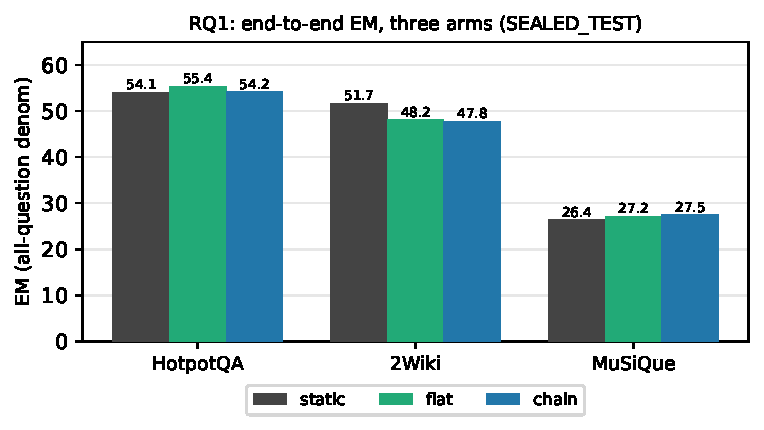
\includegraphics[width=0.62\columnwidth]{figures/fig1_em_overall.pdf}
\caption{RQ1: end-to-end EM under the all-question denominator, three arms.}
\label{fig:em_overall}
\end{figure}

\begin{figure}[t]
\centering
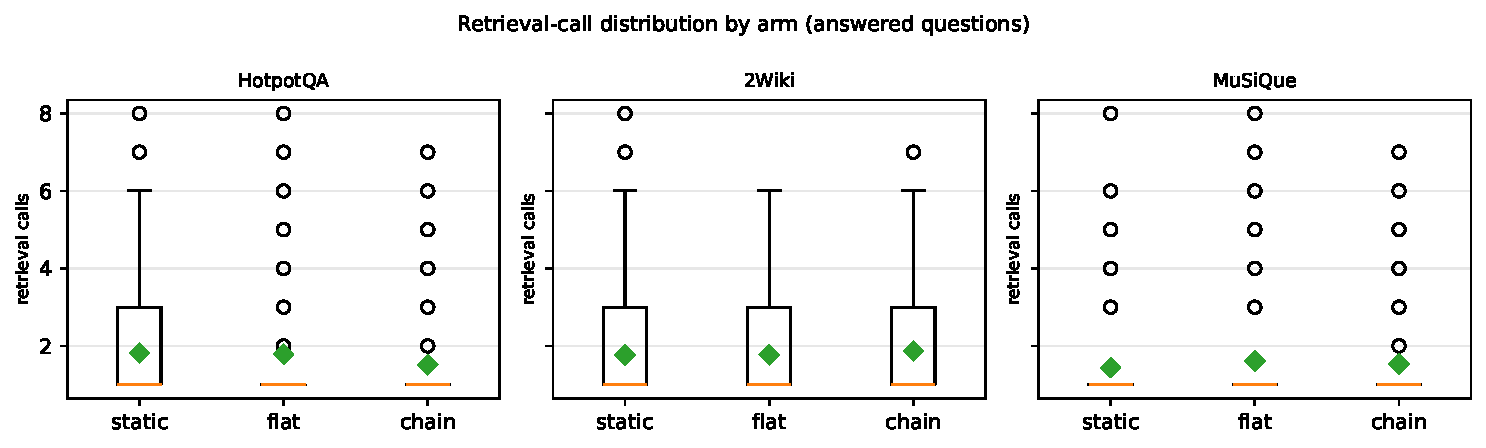
\includegraphics[width=0.92\columnwidth]{figures/fig_a_retr_dist.pdf}
\caption{RQ1/RQ2: retrieval-call distribution by arm (answered questions).
Medians are near-identical; the arms do not separate on retrieval cost.}
\label{fig:retr_dist}
\end{figure}

\begin{figure}[t]
\centering
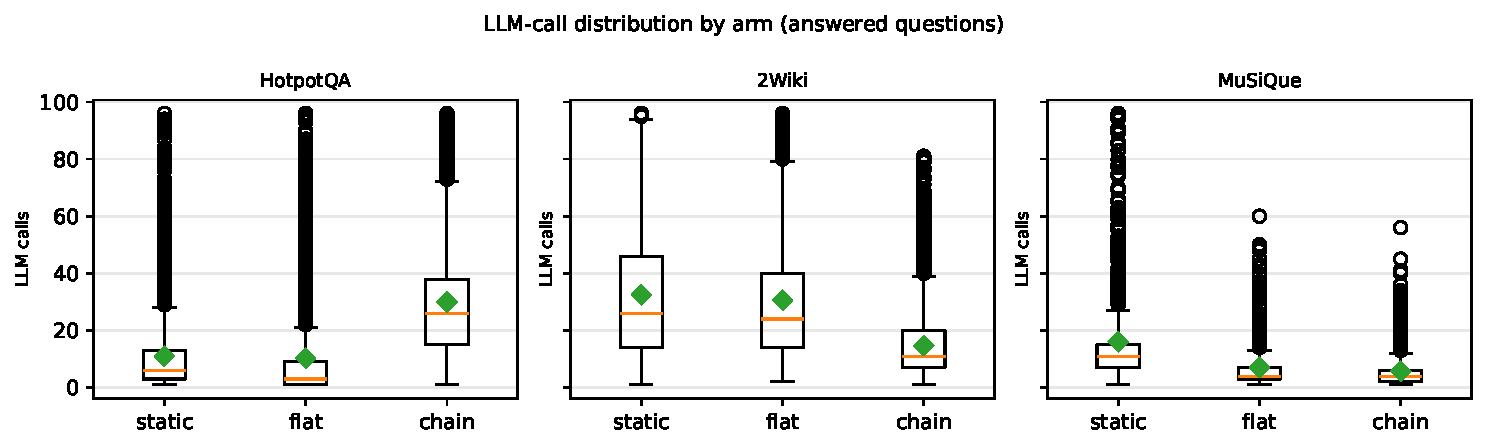
\includegraphics[width=0.92\columnwidth]{figures/fig_b_llm_dist.pdf}
\caption{RQ2: LLM-call distribution by arm. The chain arm's upper tail is
heavier on HotpotQA (more deep-exploration calls).}
\label{fig:llm_dist}
\end{figure}

\begin{figure}[t]
\centering
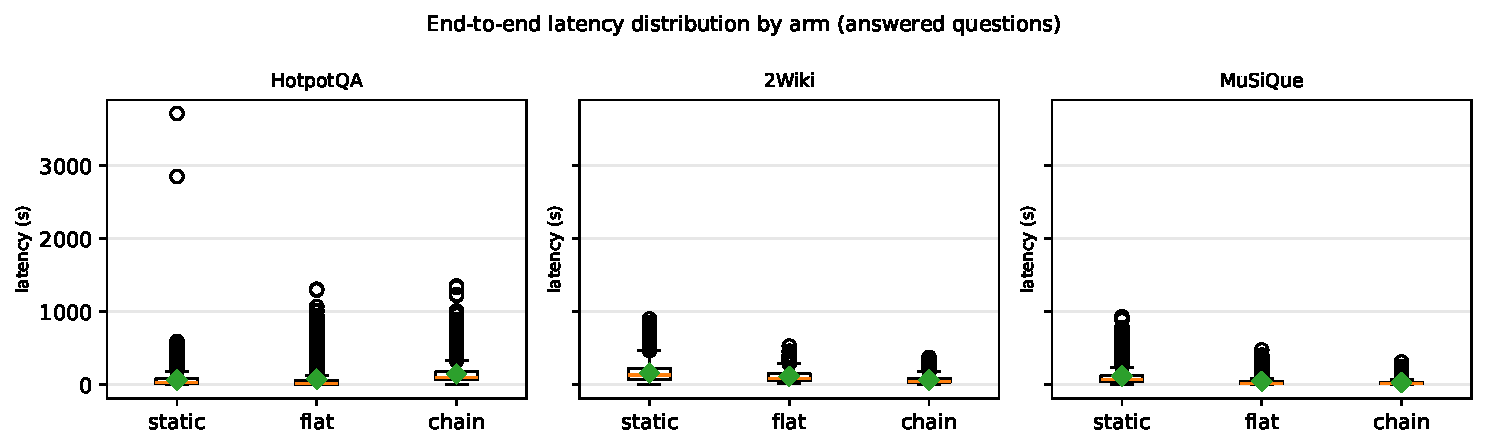
\includegraphics[width=0.92\columnwidth]{figures/fig_c_latency_dist.pdf}
\caption{RQ2: end-to-end latency distribution by arm.}
\label{fig:latency_dist}
\end{figure}

\begin{figure}[t]
\centering
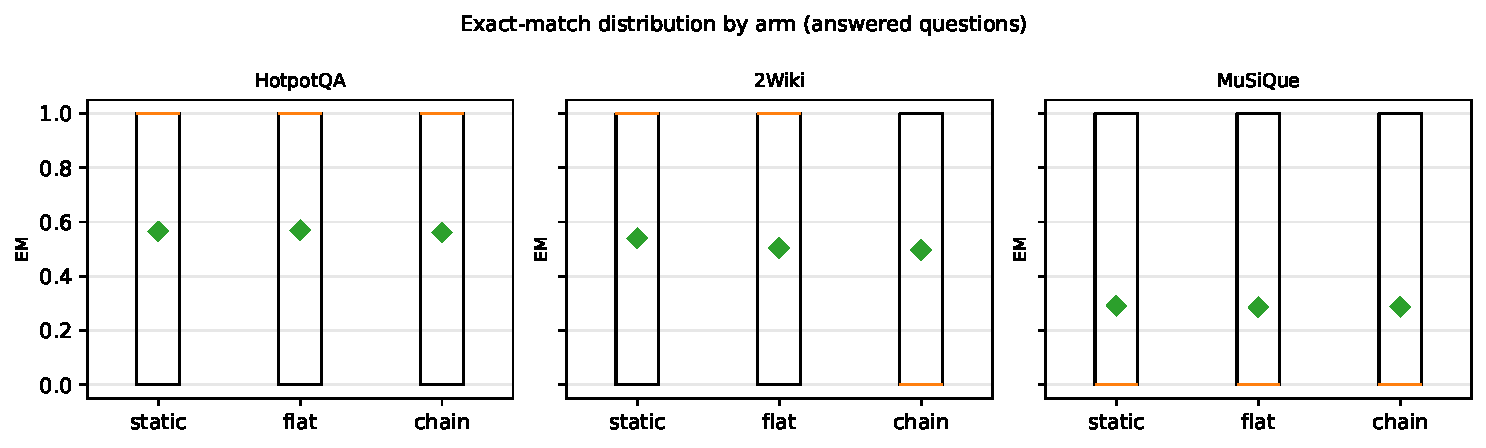
\includegraphics[width=0.92\columnwidth]{figures/fig_d_em_dist.pdf}
\caption{RQ1: exact-match distribution by arm (answered questions).}
\label{fig:em_dist}
\end{figure}

\begin{figure}[t]
\centering
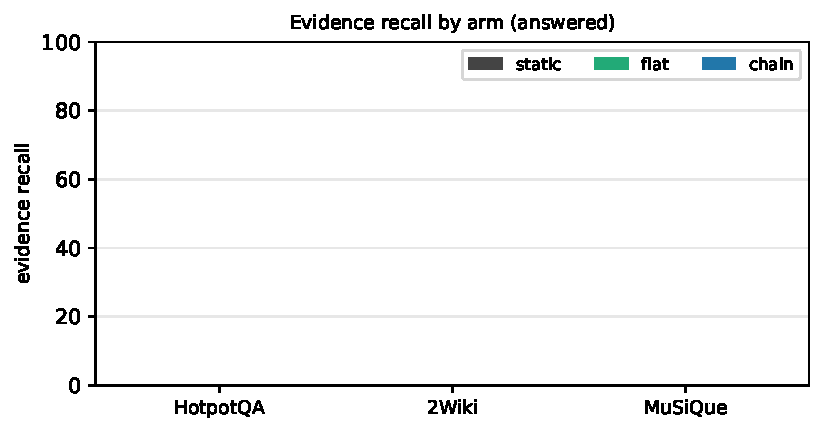
\includegraphics[width=0.55\columnwidth]{figures/fig_e_evrecall.pdf}
\caption{RQ1/RQ2: evidence recall by arm (answered questions).}
\label{fig:evrecall}
\end{figure}

\begin{figure}[t]
\centering
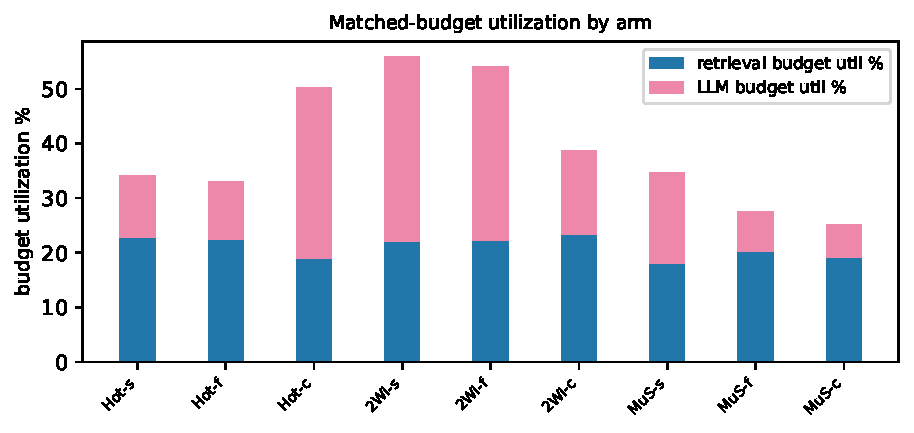
\includegraphics[width=0.72\columnwidth]{figures/fig_f_budget_util.pdf}
\caption{RQ2: matched-budget utilization (retrieval + LLM) by arm. The chain
arm consumes a larger share of its LLM budget on HotpotQA.}
\label{fig:budget_util}
\end{figure}

\begin{figure}[t]
\centering
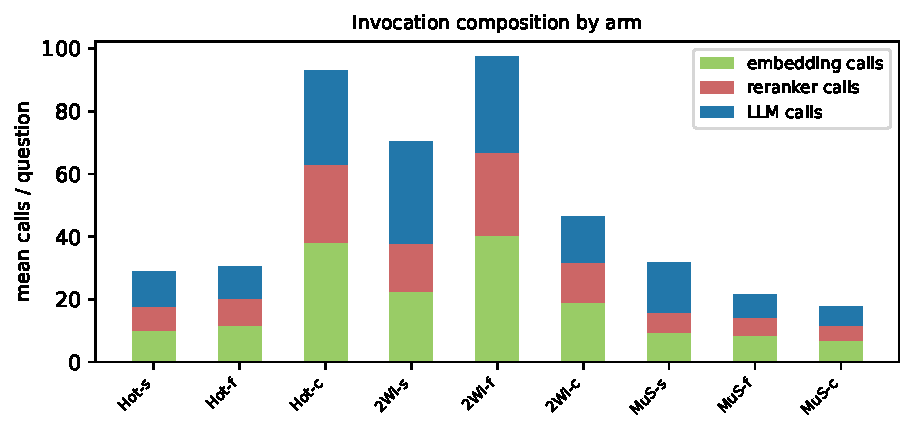
\includegraphics[width=0.72\columnwidth]{figures/fig_g_cost_comp.pdf}
\caption{RQ2: invocation composition (embedding / reranker / LLM calls) by arm.
The chain arm's extra LLM calls dominate its cost on HotpotQA.}
\label{fig:cost_comp}
\end{figure}

\subsection{Full Descriptive Statistics (supporting)}
Table~\ref{tab:descriptive} gives the complete per-arm descriptive statistics
(mean, median, p90, budget utilization, plan complexity, and invocation
counts) over the frozen SEALED\_TEST items; the numbers are machine-derived
from the run artifacts and are not hand-edited. Table~\ref{tab:paired_full}
gives the full paired chain-vs-static differences (EM, retrieval, LLM,
documents, latency) with bootstrap 95\% confidence intervals on shared
questions. Table~\ref{tab:failure_arm} breaks the execution status down by
arm and dataset, and Table~\ref{tab:evidence} reports the evidence-quality
metrics (recall, MRR, retrieved documents) by arm.

\begin{table}[t]
\centering
\caption{Full per-arm descriptive statistics on SEALED\_TEST (machine-derived
from run items; source \code{tableA\_descriptive.csv}).}
\label{tab:descriptive}
\scriptsize
\makeatletter
\begin{tabular}{llrrrrrrrrrrrr}
\toprule
dataset & arm & n & ok & budg & EM & F1 & evRec & retr & LLM & docs & lat(s) & retrU\% \\
\midrule
\@@input tables/tabA_body.tex
\bottomrule
\end{tabular}\makeatother

\end{table}

\begin{table}[t]
\centering
\caption{Paired chain-vs-static differences on shared questions, bootstrap 95\%
CI (seed 2027). Source \code{tableB\_paired.csv}.}
\label{tab:paired_full}
\scriptsize
\makeatletter
\begin{tabular}{llrrrrrr}
\toprule
dataset & metric & chain & static & $\Delta$ & CI$_{2.5}$ & CI$_{97.5}$ & n \\
\midrule
\@@input tables/tabB_body.tex
\bottomrule
\end{tabular}\makeatother

\end{table}

\begin{table}[t]
\centering
\caption{Execution status by arm $\times$ dataset (source
\code{tableC\_failure\_by\_arm.csv}).}
\label{tab:failure_arm}
\scriptsize
\makeatletter
\begin{tabular}{llrrrrrr}
\toprule
dataset & arm & ok & budget & boundary & other & total & ok\% \\
\midrule
\@@input tables/tabC_body.tex
\bottomrule
\end{tabular}\makeatother

\end{table}

\begin{table}[t]
\centering
\caption{Evidence-quality metrics by arm (source \code{tableD\_evidence.csv}).}
\label{tab:evidence}
\scriptsize
\makeatletter
\begin{tabular}{llrrrr}
\toprule
dataset & arm & evRecall & evRecall(med) & evMRR & docs \\
\midrule
\@@input tables/tabD_body.tex
\bottomrule
\end{tabular}\makeatother

\end{table}

